% Usage: knitr slide

\chapter{Correlation}\bmovie{12}\ddisc{12}
\section{Overview}

\begin{center}
\smaller
\begin{tabular}{lllll} \hline
Outcome & Predictor & Normality? & Linearity? & Analysis Method \\ \hline
Interval & Binary & Yes & & 2-sample $t$-test \textbf{or linear regression} \\
Ordinal & Binary & No & & Wilcoxon 2-sample test \\
Categorical & Categorical & & & Pearson $\chi^2$ test \\
Interval & Interval & Yes & Yes & \textbf{Correlation or linear regression} \\ 
Ordinal & Ordinal & No & No & \textbf{Spearman's rank correlation} \\ \hline
\end{tabular}\end{center}

\bi 
\item Examine association between continuous/interval outcome ($y$) and continous/interval predictor ($x$)
\item Scatterplot of $y$ versus $x$
\ei

\section{Pearson's correlation coefficient} \ros{11.1, .7-.8, .12}\katz{5.7.A}
\bi
\item $r = \frac{\Sigma(x_i - \bar{x})(y_i - \bar{y})}{\sqrt{\Sigma(x_i - \bar{x})^2\Sigma(y_i - \bar{y})^2}}$
\item Range: $-1 \leq r \leq 1$
\item Correlation coefficient is a unitless index of strength of association between two variables (+ = positive association, - = negative, 0 = no association)
\item Measures the linear relationship between $X$ and $Y$
\item Can test for significant association by testing whether the population correlation is zero
\beq
t = \frac{r\sqrt{n-2}}{\sqrt{1-r^{2}}}
\eeq
which is identical to the $t$-test used to test whether the population
$r$ is zero; d.f.=$n-2$.
\item Use probability calculator for $t$ distribution to get $P$-value
  (2-tailed if interested in association in either direction)
\item 1-tailed test for a positive correlation between $X$ and $Y$
  tests $H_{0}:$ when $X \uparrow$ does $Y \uparrow$ in the population?
\item Confidence intervals for population $r$ calculated using
  Fisher's $Z$ transformation \ros{11.8}\altman{89-91}
\beq
Z = \frac{1}{2} \textrm{log}_\textrm{e} \left( \frac{1+r}{1-r} \right)
\eeq
 \bi 
 \item For large $n$, Z follows a Normal distribution with standard error $\frac{1}{\sqrt{n-3}}$
 \item To calculate a confidence interval for $r$, first find the confidence interval for $Z$ then transform back to the $r$ scale
 \ei
\begin{eqnarray*}
 Z & = & \frac{1}{2} \textrm{log}_\textrm{e} \left( \frac{1+r}{1-r} \right) \\
 2*Z & = & \textrm{log}_\textrm{e} \left( \frac{1+r}{1-r} \right) \\
 \textrm{exp}(2*Z) & = & \left( \frac{1+r}{1-r} \right) \\
 \textrm{exp}(2*Z) * (1-r) & = & 1 + r \\
 \textrm{exp}(2*Z) - r * \textrm{exp}(2*Z) & = & 1 + r \\
 \textrm{exp}(2*Z) - 1 & = & r * \textrm{exp}(2*Z) + r \\
 \textrm{exp}(2*Z) - 1 & = & r \left(\textrm{exp}(2*Z) + 1\right) \\
 \frac{\textrm{exp}(2*Z) - 1}{\textrm{exp}(2*Z) + 1} & = & r \\
\end{eqnarray*}

 \item Example (Altman 89-90): Pearson's $r$ for a study investigating the association of basal metabolic rate with total energy expenditure was calculated to be $0.7283$ in a study of $13$ women.  Derive a 0.95 confidence interval for $r$.
\beq
 Z = \frac{1}{2} \textrm{log}_\textrm{e} \left( \frac{1+0.7283}{1-0.7283} \right) = 0.9251 \\
\eeq
The lower limit of a 0.95 CI for $Z$ is given by
\beq
  0.9251 - 1.96 * \frac{1}{\sqrt{13-3}} = 0.3053
\eeq
and the upper limit is
\beq
  0.9251 + 1.96 * \frac{1}{\sqrt{13-3}} = 1.545
\eeq
A 0.95 CI for the population correlation coefficient is given by transforming these limits from the $Z$ scale back to the $r$ scale
\beq
  \frac{\textrm{exp}(2*0.3053) - 1}{\textrm{exp}(2*0.3053) + 1} \hspace{.5cm} \textrm{to} \hspace{.5cm}  \frac{\textrm{exp}(2*1.545) - 1}{\textrm{exp}(2*1.545) + 1}
\eeq
Which gives a 0.95 CI from 0.30 to 0.91 for the population correlation
\ei
\begin{Schunk}
\begin{Sinput}
n <- 13
r <- 0.7283
z.transform <- 0.5 * log((1 + r) / (1 - r))
clz <- z.transform + c(-1, 1) * qnorm(0.975) / sqrt(n - 3)
clr <- (exp(2 * clz) - 1) / (exp(2 * clz) + 1)
round(c(z.transform, clz, clr), 4)
\end{Sinput}
\begin{Soutput}
[1] 0.9251 0.3053 1.5449 0.2962 0.9129
\end{Soutput}
\end{Schunk}

\section{Spearman's Rank Correlation}  \ros{11.12}\katz{5.7.B}
\bi
\item Pearson's $r$ assumes linear relationship between $X$ and $Y$
\item Spearman's $\rho$ (sometimes labeled $r_{s}$) assumes monotonic
  relationship between $X$ and $Y$ 
 \bi
 \item when $X \uparrow$, $Y$ always $\uparrow$ or stays flat, or $Y$
   always $\downarrow$ or stays flat
 \item does not assume linearity
 \ei
\item $\rho = r$ once replace column of $X$s by their ranks and column
  of $Y$s by ranks
\item To test $H_{0}:\rho=0$ without assuming linearity or normality,
  being damaged by outliers, or sacrificing much power (even if data are
  normal), use a $t$ statistic:
\beq
t = \frac{\rho\sqrt{n-2}}{\sqrt{1-\rho^{2}}}
\eeq
which is identical to the $t$-test used to test whether the population
$r$ is zero; d.f.=$n-2$.
\item Use probability calculator for $t$ distribution to get $P$-value
  (2-tailed if interested in association in either direction)
\item 1-tailed test for a positive correlation between $X$ and $Y$
  tests $H_{0}:$ when $X \uparrow$ does $Y \uparrow$ in the population?
\ei

\section{Correlation Examples}

\bi 
\item Correlation difficult to judge by eye
\item Example plots on following pages
\ei

\begin{Schunk}
\begin{Sinput}
# Generate 50 data points with Popluation correlations of 0, .2, .4, .6,
# .8, and .9 and plot results
require(ggplot2)
n <- 50
set.seed(123)
x <- rnorm(n, 5, 1)
d <- expand.grid(x=x, R=c(0, .2, .4, .6, .8, .9))
d <- transform(d, y = x + rnorm(nrow(d), 0,
                      ifelse(R == 0, 5, sqrt(R ^ -2 - 1))))
sfun <- function(i) {
  x <- d$x[i]; y <- d$y[i]; R <- d$R[i][1]
  r <- cor(x, y)
  tr <- r * sqrt(n - 2) / sqrt(1 - r^2)
  rho <- cor(rank(x), rank(y))
  trho <- rho * sqrt(n - 2) / sqrt(1 - rho^2)
  label <- paste('True r:', R[1], '  r:', round(r,2), '  t:', round(tr,2),
        '  rho:', round(rho,2), '  t:', round(trho,2), sep='')
  names(label) <- R
  label
  }
stats <- tapply(1 : nrow(d), d$R, sfun)
d$stats <- factor(stats[as.character(d$R)], unique(stats))
   
ggplot(d, aes(x=x, y=y)) + geom_point() + facet_wrap(~ stats) +
  theme(strip.text.x = element_text(size=7))   # Fig. (*\ref{fig:corr-corrplota}*)
\end{Sinput}
\begin{figure}[htbp]

\centerline{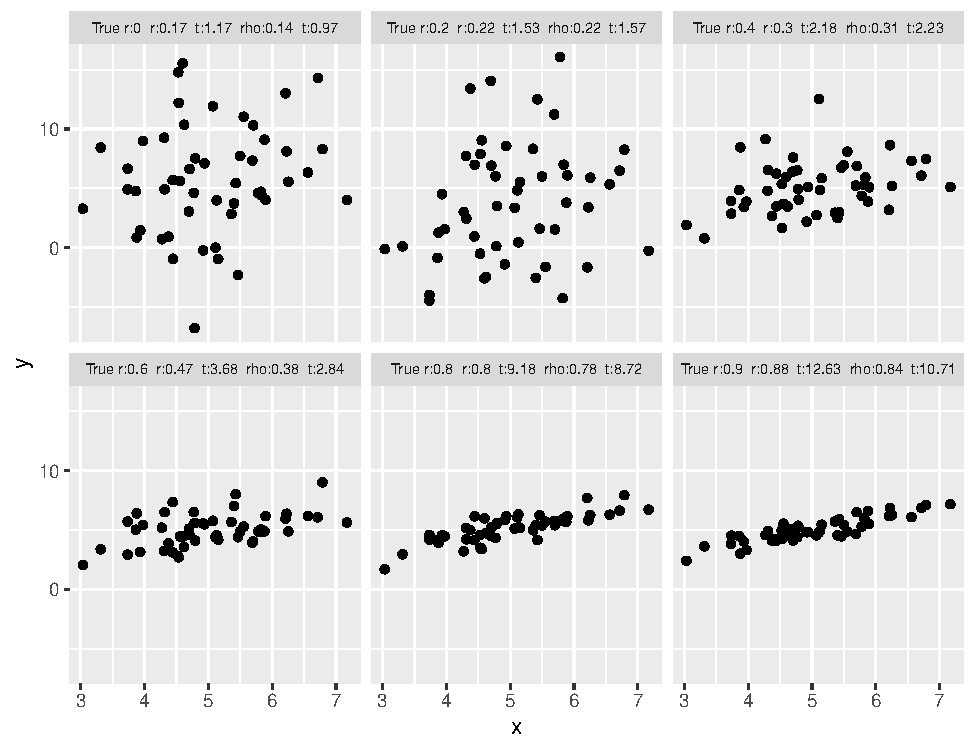
\includegraphics[width=\maxwidth]{corr-corrplota-1} }

\caption[Example correlation coefficients]{Samples of size $n=50$ for X and Y are drawn from bivariate normal populations with true correlations ranging from 0.0 to 0.9. Pearson and Spearman sample correlations are shown for samples of size 50.  Besides the population correlation coefficient, each panel is labeled with the estimated Pearson $r$, its $t$ statistic, the estimated Spearman $\rho$, and its $t$ statistic}\label{fig:corr-corrplota}
\end{figure}
\end{Schunk}
\begin{Schunk}
\begin{Sinput}
# Different scenarios that can lead to a correlation of 0.7

set.seed(123)   # Fig. (*\ref{fig:corr-corrplotb}*)
rho <- 0.7; n <- 50
var.eps <- rho^-2 - 1
x <- rnorm(n, 5, 1)
y <- x + rnorm(n, 0, sqrt(var.eps))
cor(x,y)
\end{Sinput}
\begin{Soutput}
[1] 0.6951673
\end{Soutput}
\begin{Sinput}
plot(x,y,xlab='',ylab='')

x <- c(1:20,30)
y <- c(1:20,6.2)
cor(x,y)
\end{Sinput}
\begin{Soutput}
[1] 0.6988119
\end{Soutput}
\begin{Sinput}
plot(x,y,xlab='',ylab='')

set.seed(123)
x <- rnorm(40)
y <- rnorm(40)
x[21] <- y[21] <- 8.5
cor(x,y)
\end{Sinput}
\begin{Soutput}
[1] 0.7014825
\end{Soutput}
\begin{Sinput}
plot(x,y,xlab='',ylab='')

x <- rep(0:19,2)
y <- c(rep(.62,20),rep(2,20)) * x
cor(x,y)
\end{Sinput}
\begin{Soutput}
[1] 0.701783
\end{Soutput}
\begin{Sinput}
plot(x,y,xlab='',ylab='')

x <- -7:12
y <- x^2
cor(x,y)
\end{Sinput}
\begin{Soutput}
[1] 0.6974104
\end{Soutput}
\begin{Sinput}
plot(x,y,xlab='',ylab='')

set.seed(123)
tmp <- 1:20 / 2
x <- c(rnorm(20, tmp, 1), tmp + rnorm(20,14.5,1))
y <- c(rnorm(20, -tmp, 1), -tmp + rnorm(20,14.5,1))
cor(x,y)
\end{Sinput}
\begin{Soutput}
[1] 0.703308
\end{Soutput}
\begin{Sinput}
plot(x,y,xlab='',ylab='')
\end{Sinput}
\begin{figure}[htbp]

\centerline{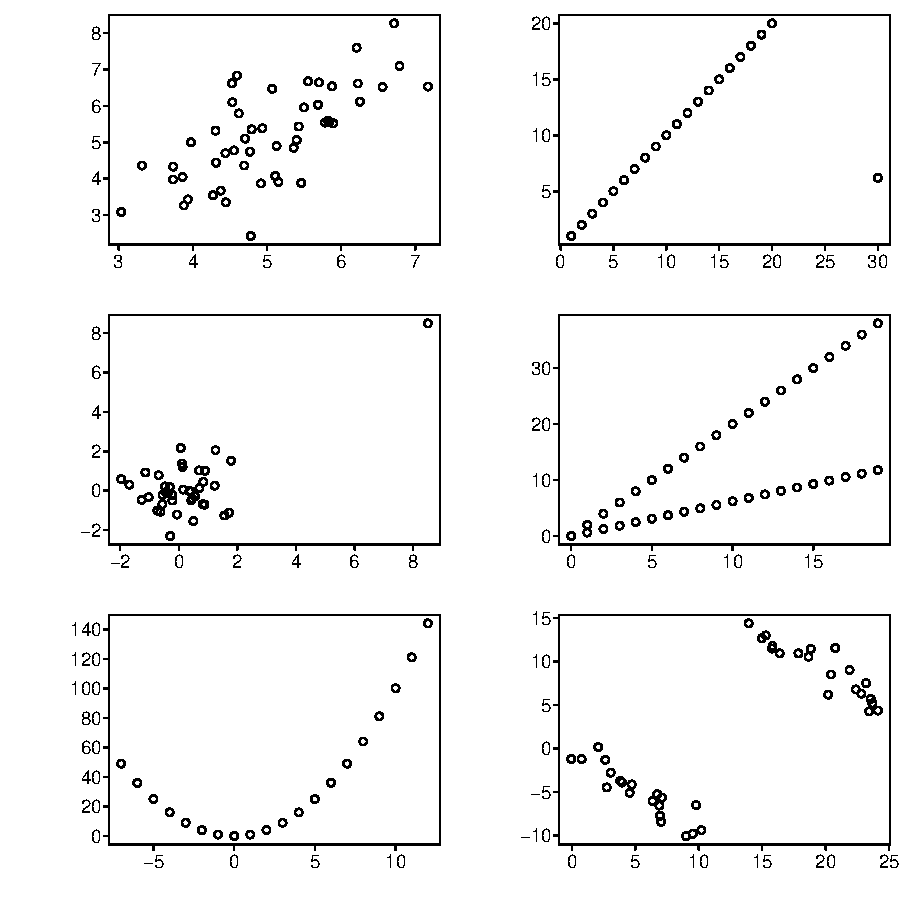
\includegraphics[width=\maxwidth]{corr-corrplotb-1} }

\caption[Multiple datasets having same Pearson $r$]{Different observed datasets that have the same correlation.  All six plots have a sample Pearson correlation of $0.7$.}\label{fig:corr-corrplotb}
\end{figure}
\end{Schunk}


\clearpage
\section{Correlation and Agreement}

\bi 
 \item Compare two methods of measuring the same underlying value
  \bi 
  \item Lung function measured using a spirometer (expensive, accurate) or peak flow meter (cheap, less accurate)
  \item Two devices (oropharyngeal and conventional) used to mesured
    acidity (pH) in the esophagus as a marker of reflux
  \ei
 \item Typical (incorrect) approach begins with scatterplot of one
   method vs.\ the other with a 1:1 line indicating perfect agreement
 \item See Figure~\ref{fig:descript-pH}
 \item Incorrect approach would report a high correlation ($r = 0.90$) and conclude good agreement
 \item Problems with the correlation approach
  \begin{enumerate}
   \item $r$ measures the degree of linear association between two
     variables, not the agreement.  If, for example, the Sandhill
     consistently gave pH values that were 0.5 unit higher than the
     Restech, we could still have high correlation, but poor agreement
     between the two devices.  We can have high correlation if the two
     devices lie closely to any line, not just a 1:1 line that
     indicates perfect agreement.  
   \item A change in scale does not affect correlation, but does
     influence agreement. For example, if the Sandhill always
     registered 2 times larger than the Restech, we would have perfect
     correlation but the agreement would get progressively worse for
     larger values of pH. 
   \item Correlation depends on the range of the data so that larger
     ranges lead to larger correlations.  This can lead to vary
     strange interpretations 

\begin{table}[!h]
\begin{center}
\begin{tabular}{l|cc}
 & $r$ & $\rho$ \\ \hline
all data & 0.90 & 0.73 \\ 
avg pH $\leq 4$ & 0.51 & 0.58 \\ 
avg pH $> 4$ & 0.74 & 0.65
\end{tabular}
\caption{Pearson ($r$) and Spearman ($\rho$) correlations for Restech and Sandhill pH data.  The correlation calculated using all of the data is larger than the correlation calculated using a retricted range of the data.  However, it would be difficult to claim that the overall agreement is better than both the agreement when pH is less than 4 and when pH is greater than 4.}
\end{center}
\end{table}

\item Tests of significance (testing if $r=0$) are irrelevant to the
  question at hand, but often reported to demonstrate a significant
  association.  The two devices are measuring the same quantity, so it
  would be shocking if we did not observe a highly significant
  $p$-value. A $p < .0001$ is not impressive.  A regression analysis
  with a highly significant slope would be similarly unimpressive. 
\item Data can have high correlation, but poor agreement.  There are
  many examples in the literature, but even in our analysis with $r =
  0.90$, the correlation is high, but we will show that the agreement
  is not as good as the high correlation implies. \
  \end{enumerate}
\ei

See Chapter~\ref{chap:obsvar} for simple approaches to assessing agreement
and analyzing observer variability studies.

\subsection{Bland-Altman Plots} \ems{36.4}

\bi 
  \item See Bland and Altman (1986, Lancet)
  \item Earlier: Tukey mean-difference plot
  \item Create plots of the difference in measurements on the y-axis
    versus the average value of the two devices on the x-axis 
  \item If the two devices agree, the difference should be about zero
  \item The average of the two devices is our best estimate of the
    true, unknown (pH) value that is we are trying to measure 
  \item Measurements will often vary in a systematic way over the
    range of measurement. By plotting the difference versus the
    average, we can visually determine if the difference changes over
    our estimate of the truth. 
  \item Solid line indicated the mean, dashed lines are approximate
    0.95 confidence intervals (assuming Normality) 
\ei

\textbf{But} there is controversy about what should be on the $x$-axis
of the plot.  Krouwer~\cite{kro08why} concluded that:
\bi
\item When the two measures have nearly equal variability, i.e., when
  comparing two ``field measurements'', the Bland-Altman approach is preferred
\item When one measurement is a ``reference standard'' having much less
  variation than the field measurement, the reference standard and not
  the average of the two measurements should be on the $x$-axis
\ei

\begin{Schunk}
\begin{Sinput}
require(Hmisc)
getHdata(esopH)
esopH$diff <- with(esopH, orophar - conv)
ggplot(esopH, aes(x=(conv + orophar)/2, y=diff)) +   # Fig. (*\ref{fig:corr-baplot}*)
  stat_binhex(aes(alpha=..count.., color=Hmisc::cut2(..count.., g=20)),
              bins=80) +
  stat_smooth() +
  geom_hline(yintercept = mean(esopH$diff, na.rm=TRUE) +
   c(-1.96, 0, 1.96) * sd(esopH$diff, na.rm=TRUE),
   linetype=c(2,1,2), color='brown') +
  xlab('Average of Conventional and Oropharyngeal pH') +
  ylab('Oropharyngeal Minus Conventional pH') +
  guides(alpha=FALSE, fill=FALSE, color=guide_legend(title='Frequency'))
\end{Sinput}
\begin{figure}[htbp]

\centerline{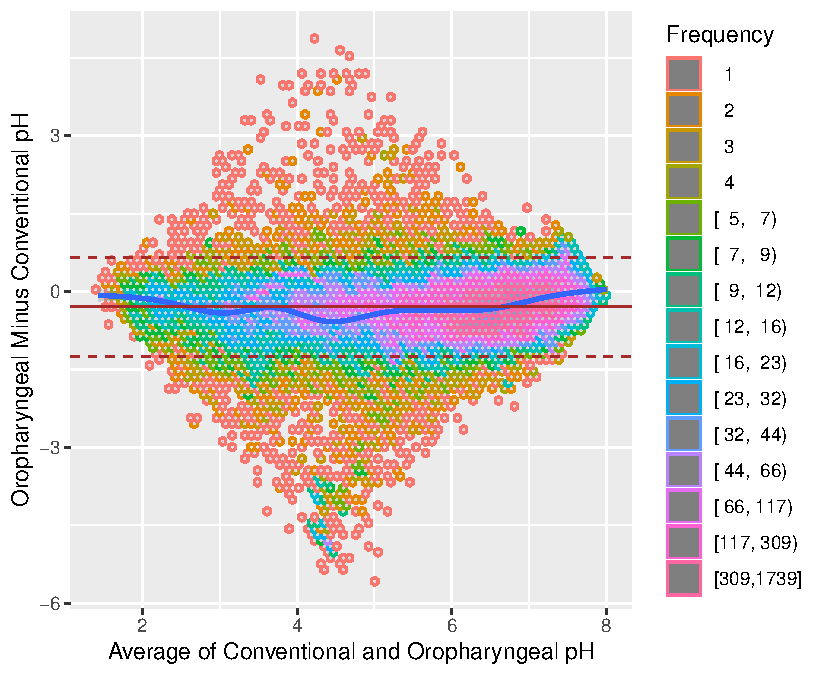
\includegraphics[width=\maxwidth]{corr-baplot-1} }

\caption[Bland-Altman plot for 2 pH measurements]{Bland-Altman plot for the oroesophageal and conventional pH measurements, using hexagonal binning because of the large sample size.  The difference in pH mesaurements (oro.\ -conventional) is presented on the $y$-axis and the average of the two devices on the $x$-axis.  We see poor agreement around pH values of 4-5}\label{fig:corr-baplot}
\end{figure}
\end{Schunk}

\bi 
  \item We will also consider differences in the two measurements over the time of day
  \item The added smooth curve is called a locally weighted scatterplot smooth (loess)
\ei

\begin{Schunk}
\begin{Sinput}
getHdata(esopH2)
ggplot(esopH2, aes(x=time, y=diffpH)) +    # Fig. (*\ref{fig:corr-phtimediff}*)
       geom_point(pch='.') + stat_smooth() +
       geom_hline(yintercept = 0, col='gray60') +
       scale_x_continuous(breaks=seq(16, 38, by=4),
                          labels=c("4 PM", "8 PM", "12 AM",
                            "4 AM", "8AM", "12 PM"),
                          limits=c(14, 14+24)) +
       ylab('Average of Oropharyngeal Minus Conventional pH') +
       xlab('Time of Day')
\end{Sinput}
\begin{figure}[htbp]

\centerline{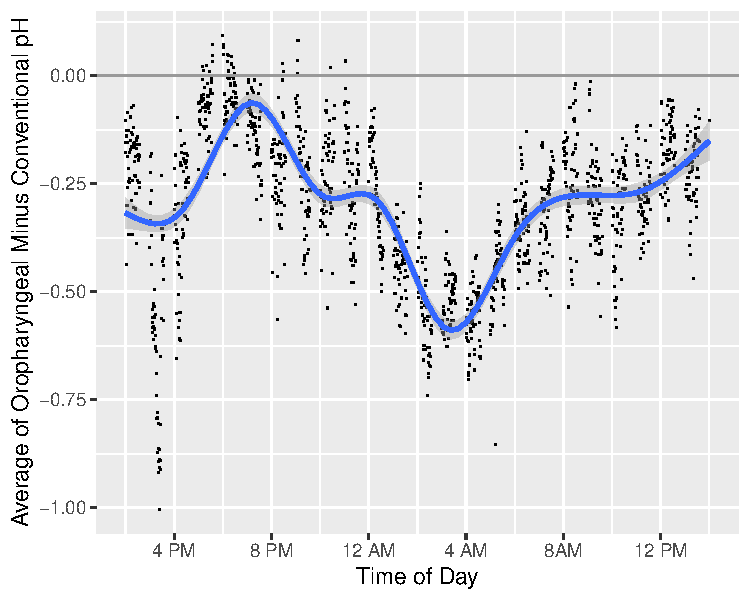
\includegraphics[width=\maxwidth]{corr-phtimediff-1} }

\caption[Difference in pH by time of day]{Difference in pH measurements (oro. - conventional) by time of day along with a loess smoother and pointwise 0.95 confidence bands.  Is the difference modified by a subject being in a supine position rather than being upright?}\label{fig:corr-phtimediff}
\end{figure}
\end{Schunk}

\subsection{Sample Size for $r$}\alabel{sec:corr-n}
\bi
\item Without knowledge of population variances, etc., $r$ can be
  useful for planning studies
\item Choose $n$ so that margin for error (half-width of C.L.) for $r$
  is acceptable
\item Precision of $r$ in estimating $\rho$ is generally worst when $\rho=0$
\item This margin for error as well as that for three other choices of the unknown true $\rho$ are shown in Figure~\ref{fig:corr-moe}.
\begin{Schunk}
\begin{Sinput}
require(Hmisc)
plotCorrPrecision(rho=c(0, .25, .5, .75),
                  n=seq(10, 1000, length=100),
                  ylim=c(0, .4), col=1:4, opts=list(keys='lines'))
abline(h=seq(0, .4, by=0.025),
       v=seq(25, 975, by=25), col=gray(.9))
\end{Sinput}
\begin{figure}[htbp]

\centerline{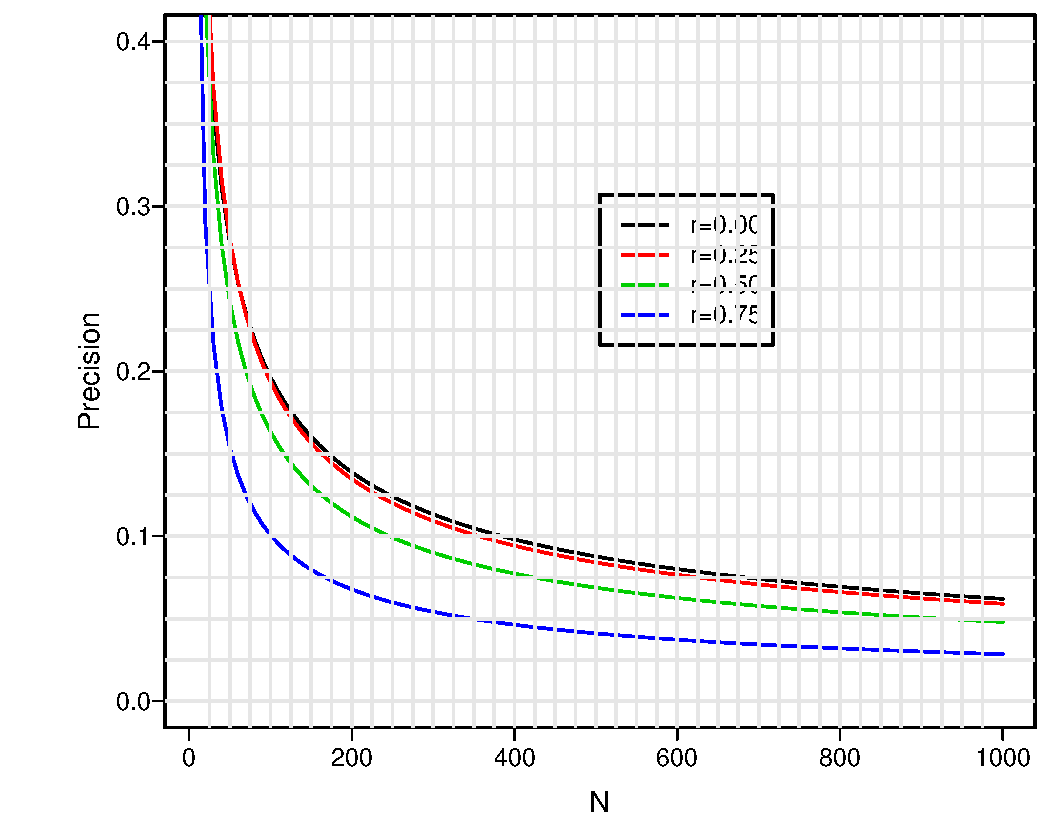
\includegraphics[width=\maxwidth]{corr-moe-1} }

\caption[Margin of error for estimating correlation coefficient]{Margin for error (length of longer side of asymmetric 0.95 confidence interval) for $r$ in estimating $\rho$, when $\rho=0, 0.25, 0.5, 0.75$.  Calculations are based on Fisher $z$ transformation of $r$.}\label{fig:corr-moe}
\end{figure}
\end{Schunk}
\ei

See also \href{https://stats.stackexchange.com/questions/415131}{stats.stackexchange.com/questions/415131}.

\subsection{Comparing Two $r$'s}
\bi
\item Rarely appropriate
\item Two $r$'s can be the same even though slopes may differ
\item Usually better to compare effects on a real scale (slopes)
\ei

\section{Avoiding Overinterpretation}
\bi
\item Often researchers 
 \bi
 \item compute many correlations then
 \item make a big deal out of the largest observed correlation
 \ei
\item This is \emph{double dipping}: using the same dataset to tell you which features to test, then testing those features
\item This is a ranking and selection problem, and the data seldom contain enough information to be reliable in the choices
\ei

\subsection{Simulate Data}
\bi
\item For our analysis experiments, simulate a sample of size 50 from a 10-variate normal distribution with a known correlation matrix
\item To specify this correlation matrix take the easy way out: compute an observed correlation matrix from a small sample where all correlations in the population are zero
\item The usual sample noise will generate some large observed correlations
\begin{Schunk}
\begin{Sinput}
require(Hmisc)
require(mvtnorm)
\end{Sinput}
\begin{Sinput}
# Get a population correlation matrix by getting sample correlations
# on a random normal sample with N=20 and all true correlations=0
# then pretend these sample correlations were real population values
set.seed(3)
x <- rmvnorm(20, sigma=diag(10))
R <- rcorr(x)$r
# True correlations we will simulate from:
round(R, 2)
\end{Sinput}
\begin{Soutput}
       [,1]  [,2]  [,3]  [,4]  [,5]  [,6]  [,7]  [,8]  [,9] [,10]
 [1,]  1.00  0.01  0.47 -0.09 -0.31 -0.07  0.14  0.05  0.02 -0.49
 [2,]  0.01  1.00  0.48  0.27  0.27  0.14  0.40 -0.17 -0.59  0.60
 [3,]  0.47  0.48  1.00 -0.11  0.26 -0.31  0.45 -0.12 -0.50 -0.06
 [4,] -0.09  0.27 -0.11  1.00  0.42  0.42 -0.07 -0.35  0.16  0.35
 [5,] -0.31  0.27  0.26  0.42  1.00 -0.04  0.03 -0.40 -0.25  0.34
 [6,] -0.07  0.14 -0.31  0.42 -0.04  1.00  0.19 -0.36  0.08  0.40
 [7,]  0.14  0.40  0.45 -0.07  0.03  0.19  1.00 -0.37 -0.65 -0.07
 [8,]  0.05 -0.17 -0.12 -0.35 -0.40 -0.36 -0.37  1.00  0.17 -0.24
 [9,]  0.02 -0.59 -0.50  0.16 -0.25  0.08 -0.65  0.17  1.00 -0.18
[10,] -0.49  0.60 -0.06  0.35  0.34  0.40 -0.07 -0.24 -0.18  1.00
\end{Soutput}
\begin{Sinput}
# Get a huge sample from a multivariate normal distribution to see
# that it mimics the real correlation matrix R
x <- rmvnorm(50000, sigma=R)
table(round(R - rcorr(x)$r, 2))
\end{Sinput}
\begin{Soutput}

-0.01     0  0.01 
   14    76    10 
\end{Soutput}
\begin{Sinput}
# Now sample from the population to get our dataset with N=50
x <- rmvnorm(50, sigma=R)
rorig <- rcorr(x)$r
round(rorig, 2)
\end{Sinput}
\begin{Soutput}
       [,1]  [,2]  [,3]  [,4]  [,5]  [,6]  [,7]  [,8]  [,9] [,10]
 [1,]  1.00 -0.01  0.50  0.11  0.00 -0.16  0.07 -0.04 -0.04 -0.43
 [2,] -0.01  1.00  0.50  0.19  0.43  0.13  0.60 -0.26 -0.76  0.69
 [3,]  0.50  0.50  1.00 -0.15  0.45 -0.41  0.52 -0.18 -0.58 -0.01
 [4,]  0.11  0.19 -0.15  1.00  0.45  0.30 -0.13 -0.35  0.09  0.14
 [5,]  0.00  0.43  0.45  0.45  1.00 -0.12  0.27 -0.53 -0.42  0.20
 [6,] -0.16  0.13 -0.41  0.30 -0.12  1.00  0.06 -0.27  0.00  0.51
 [7,]  0.07  0.60  0.52 -0.13  0.27  0.06  1.00 -0.57 -0.81  0.19
 [8,] -0.04 -0.26 -0.18 -0.35 -0.53 -0.27 -0.57  1.00  0.37 -0.13
 [9,] -0.04 -0.76 -0.58  0.09 -0.42  0.00 -0.81  0.37  1.00 -0.41
[10,] -0.43  0.69 -0.01  0.14  0.20  0.51  0.19 -0.13 -0.41  1.00
\end{Soutput}
\end{Schunk}
\ei

\subsection{Margin of Error for a Single $r$}
\bi
\item First compute the margin of error in estimating a single $r$ from $n=50$
\item This is the spacing between $r$ and it's lower 0.95 CL or the spacing between $r$ and its upper CL whichever is greatest
\item CL based on Fisher's $z$-transformation described earlier
\item Compute this for 4 hypothetical true $r$: 0 0.25 0.5 0.75
\begin{Schunk}
\begin{Sinput}
r <- (0 : 3) / 4
n <- 50
zcrit <- qnorm(0.975)
z <- 0.5 * log( (1 + r) / (1 - r))
lo <- z - zcrit/sqrt(n-3)
hi <- z + zcrit/sqrt(n-3)
rlo <- (exp(2*lo)-1)/(exp(2*lo)+1)
rhi <- (exp(2*hi)-1)/(exp(2*hi)+1)
w <- rbind(r=r, 'Margin of Error'=pmax(rhi - r, r - rlo))
prmatrix(round(w, 2), collab=rep('', 4))
\end{Sinput}
\begin{Soutput}
                                   
r               0.00 0.25 0.50 0.75
Margin of Error 0.28 0.28 0.24 0.15
\end{Soutput}
\end{Schunk}
\item If the true correlation is 0.5, the margin of error in estimating it is $\pm 0.24$ with $n=50$
\ei

\subsection{Bootstrapping the Correlation Selection Process}
\bi
\item Can use the bootstrap to document the difficulty of the task
\item Steps:
 \be 
 \item form a matrix with $N$ rows and $p$ columns where $N$ is the number of observations and $p$ is the number of variables being correlated with each other
 \item draw a sample of size $N$ from this matrix by sampling its rows
 \item compute all the correlation coefficients as was done previously
 \item re-run the same selection process as was done on the original dataset
 \item repeat 1000 times
 \item examine the distribution of the selections over the 1000 repeats
 \ee
\ei

\subsection{Bootstrapping Bias in Largest Observed $r$}
\bi
\item Start with something simpler than ranking all the $r$s in the matrix: estimate the bias in the largest observed $r$
\item Draw a sample with replacement from rows of the data matrix
\item For each of these bootstrap samples find which pair of variables has the highest $r$
\item Track this variable pair and compute $r$ in the original sample
\item Compute the dropoff in $r$ from the bootstrap sample to the original sample
\item This simulates the \emph{process} used to find the largest $r$
\item Example: use data simulated above with 10 standard normal random variables \& known correlation matrix on 50 subjects
\item Sample correlation matrix has $\frac{10 \times 9}{2} = 45$ distinct coefficients
\begin{Schunk}
\begin{Sinput}
# Function to retrieve the upper triangle of a symmetric matrix
# ignoring the diagnonal terms
up <- function(z) z[upper.tri(z)]
rorigu <- up(rorig)
max(rorigu)   # .685 = [2,10] element; 0.604 in population
\end{Sinput}
\begin{Soutput}
[1] 0.6854261
\end{Soutput}
\begin{Sinput}
which.max(rorigu)
\end{Sinput}
\begin{Soutput}
[1] 38
\end{Soutput}
\begin{Sinput}
# is the 38th element in the upper triangle

# Tabulate the difference between sample r estimates and true values
Ru <- up(R)
mean(abs(Ru - rorigu))
\end{Sinput}
\begin{Soutput}
[1] 0.1149512
\end{Soutput}
\begin{Sinput}
table(round(Ru - rorigu, 1))
\end{Sinput}
\begin{Soutput}

-0.3 -0.2 -0.1    0  0.1  0.2 
   2    6    7    7   17    6 
\end{Soutput}
\begin{Sinput}
# Repeat the "finding max r" procedure for 1000 bootstrap samples
# Sample from x 1000 times with replacement, each time computing
# a new correlation matrix
samepair <- dropsum <- 0
for(i in 1 : 1000) {
  b  <- sample(1 : 50, replace=TRUE)
  xb <- x[b, ]   # sample with replacement from rows
  r  <- rcorr(xb)$r
  ru <- up(r)
  wmax <- which.max(ru)
  if(wmax == 38) samepair <- samepair + 1
  # Compute correlation for the bootstrap best pair in the original sample
  origr <- rorigu[wmax]
  # Compute dropoff in best r
  dropoff <- ru[wmax] - origr
  dropsum <- dropsum + dropoff
}
cat('Number of bootstaps selecting the original most correlated pair:',
    samepair, 'out of 1000', '\n')
\end{Sinput}
\begin{Soutput}
Number of bootstaps selecting the original most correlated pair: 642 out of 1000 
\end{Soutput}
\begin{Sinput}
cat('Mean dropoff for max r:', round(dropsum / 1000, 3), '\n')
\end{Sinput}
\begin{Soutput}
Mean dropoff for max r: 0.071 
\end{Soutput}
\end{Schunk}

\item For our dataset with $n=50$ we expect that the maximum observed $r$ out of 45 $r$s is biased high by 0.071
 \bi
 \item Could subtact 0.071 to debias the observed max $r$ although this will worsen its precision
 \ei
\ei

\subsection{Bootstrapping Ranks of All $r$s}
\bi
\item Do a more comprehensive assessment that quantifies the difficulty of the task in ranking all the $r$s
\item Quantity uncertainties in the ranks of the original correlation coefficients
\item Apparent ``winner'' was the one receiving the highest ranking
  $q$ among all $r$s
\item What is the distribution of $q$ over the 1000 bootstrap samples?
\item Can easily compute a 0.95 bootstrap nonparametric percentile confidence interval for the true unknown ranking of that feature combination and for ranking all the examined feature correlations
\item Bootstrap the correlation matrix and re-rank the coefficients
\item For each pair of variables compute the 0.95 confidence interval for the rank of its correlation from among the 45

\begin{Schunk}
\begin{Sinput}
# For each observed correlation compute its rank among 45 distinct pairs
orig.ranks <- rank(up(rorig))
# Sample from x 1000 times with replacement, each time computing
# a new correlation matrix
Rm <- matrix(NA, nrow=1000, ncol=45)
for(i in 1 : 1000) {
  b  <- sample(1 : 50, replace=TRUE)
  xb <- x[b, ]
  r  <- rcorr(xb)$r
  Rm[i, ] <- rank(up(r))
}
# Over bootstrap correlations compute quantiles of ranks
low  <- apply(Rm, 2, quantile, probs=0.025)
high <- apply(Rm, 2, quantile, probs=0.975)
round(cbind('Original Rank'=orig.ranks, Lower=low, Upper=high))
\end{Sinput}
\begin{Soutput}
      Original Rank Lower Upper
 [1,]            22    12    34
 [2,]            40    32    45
 [3,]            41    30    45
 [4,]            28    15    37
 [5,]            31    20    38
 [6,]            15     8    28
 [7,]            24    11    34
 [8,]            37    32    43
 [9,]            38    32    43
[10,]            39    31    44
[11,]            14     8    27
[12,]            29    15    37
[13,]             9     3    15
[14,]            35    22    43
[15,]            18    10    26
[16,]            26    16    34
[17,]            44    38    45
[18,]            43    34    45
[19,]            16     9    27
[20,]            34    25    38
[21,]            25    14    34
[22,]            19    11    32
[23,]            12     7    21
[24,]            13     7    27
[25,]            10     4    20
[26,]             5     3    10
[27,]            11     5    22
[28,]             4     3     8
[29,]            20    10    33
[30,]             2     1     4
[31,]             3     2    11
[32,]            27    16    36
[33,]             7     4    13
[34,]            23    13    32
[35,]             1     1     2
[36,]            36    28    43
[37,]             6     3    15
[38,]            45    40    45
[39,]            21    12    31
[40,]            30    17    37
[41,]            33    21    39
[42,]            42    34    44
[43,]            32    20    38
[44,]            17    11    28
[45,]             8     3    16
\end{Soutput}
\end{Schunk}

\item Highest observed $r$ (rank 45) has 0.95 CI $[40,45]$
\item Data are consistent with it being the $6^\textrm{th}$ highest
\item Smallest observed value (rank 1; most impressive negative
  correlation) has CI $[1, 2]$ for rank; data consistent with that
  pair of variables being the best or $2^\textrm{nd}$
\item The $r$ originally ranked $36^\textrm{th}$ has a 0.95 CI of $[28, 43]$ so the data are consistent with it being in the top 3
\ei

\subsection{Monte Carlo Simulation to Get A Rank Interval}
\bi
\item For comparison with the bootstrap, get the frequency distribution of ranks in repeated studies of the apparently highest $r$ in our $n=50$ study
\item Repeated studies will also have $n=50$ and will be generated from the population correlation matrix
\item Recall that original max $r$ was the $38^\textrm{th}$ element of the strung-out $r$ matrix from our sample
\begin{Schunk}
\begin{Sinput}
ranks <- integer(1000)
for(i in 1 : 1000) {
  xs <- rmvnorm(50, sigma=R)
  rsim <- up(rcorr(xs)$r)
  ranks[i] <- rank(rsim)[38]
}
table(ranks)   # freqs. of ranks of 38th element in new samples
\end{Sinput}
\begin{Soutput}
ranks
 34  35  36  37  38  39  40  41  42  43  44  45 
  2   1   6   8  10  18  25  38  58  88 152 594 
\end{Soutput}
\begin{Sinput}
quantile(ranks, c(0.025, 0.975))
\end{Sinput}
\begin{Soutput}
 2.5% 97.5% 
   38    45 
\end{Soutput}
\end{Schunk}
\item This interval is a bit wider than the bootstrap interval
\item \textbf{Note}: both the bootstrap and the Monte Carlo simulated interval would be \textbf{far wider} had the number of correlation coefficients estimated been much greater than the sample size
\item Example: consider 1000 possible associations with a single $Y$
\item This time the potential predictors $X$ will be independent in the population and they will be conditioned on (held constant over simulations at the original $X$ values)
\item The true importance of the $X$s is $1, 2, \ldots, 10$ for the first 10 and all remaining are irrelevant in the population
\begin{Schunk}
\begin{Sinput}
set.seed(8)
n <- 50
p <- 1000
x <- matrix(rnorm(n * p), ncol=p)
Ey <- x[,1] + 2 * x[,2] + 3 * x[,3] + 4 * x[,4] + 5 * x[,5] + 6 * x[,6] +
      7 * x[,7] + 8 * x[,8] + 9 * x[,9] + 10 * x[,10]
y <- Ey + rnorm(n) * 20
ro <- cor(x, y)
# First 10 correlations and tabulate all others
round(ro[1:10], 2)
\end{Sinput}
\begin{Soutput}
 [1]  0.26 -0.16  0.05  0.29 -0.03  0.04  0.28  0.05  0.28  0.57
\end{Soutput}
\begin{Sinput}
table(round(ro[-(1:10)], 1))
\end{Sinput}
\begin{Soutput}

-0.5 -0.4 -0.3 -0.2 -0.1    0  0.1  0.2  0.3  0.4  0.5 
   1    6   43   97  234  250  210  120   25    3    1 
\end{Soutput}
\begin{Sinput}
# Find which of the 1000 correlation against Y is largest
wmax <- which.max(ro)
wmax     # correct according to population
\end{Sinput}
\begin{Soutput}
[1] 10
\end{Soutput}
\begin{Sinput}
ro[wmax]   # original rank=1000
\end{Sinput}
\begin{Soutput}
[1] 0.5698995
\end{Soutput}
\begin{Sinput}
# Simulate 1000 repeats of sample with new y but keeping x the same
# See how original highest correlating variable ranks among 1000
# correlations in new samples

ranks <- numeric(1000)
for(i in 1 : 1000) {
  ys <- Ey + rnorm(n) * 20
  rs <- cor(x, ys)
  ranks[i] <- rank(rs)[wmax]
}

table(round(ranks, -1))   # round to nearest 10
\end{Sinput}
\begin{Soutput}

 350  400  580  600  610  620  630  660  670  680  690  700  710  720  730  740 
   1    1    1    1    1    2    1    1    4    2    2    2    1    2    1    1 
 760  770  780  790  800  810  820  830  840  850  860  870  880  890  900  910 
   1    1    2    4    6    2    6   11    3    6    6    9   13    8   15   15 
 920  930  940  950  960  970  980  990 1000 
  15   34   39   41   50   66  126  203  294 
\end{Soutput}
\begin{Sinput}
quantile(ranks, c(0.025, 0.975))
\end{Sinput}
\begin{Soutput}
   2.5%   97.5% 
 770.85 1000.00 
\end{Soutput}
\begin{Sinput}
sum(ranks > 998)
\end{Sinput}
\begin{Soutput}
[1] 139
\end{Soutput}
\end{Schunk}

\item The apparent winning variable could fairly easily be the $771^\textrm{st}$ largest instead of the $1000^\textrm{th}$ ranked correlation
\item The winning variable was in the top two in only 139 out of 1000 simulations
\item See Chapter~\ref{chap:hdata} for more ways to quantify limitations of high-dimensional data analysis, including the $p > N$ case
\ei
